\documentclass[slide]{../../custom}
\begin{document}

\begin{frame}
  \titlepage
\end{frame}

\begin{frame}
  \frametitle{摘要}
  \begin{itemize}
    \item \textbf{论文阅读与对比分析}
    \item \textbf{创新方向确定}
    \item \textbf{论文写作}
  \end{itemize}
\end{frame}

\begin{frame}
  \frametitle{论文创新点对比}
  为扩展研究视角并探索创新方向,在深入研读了 \cite{Wang2025} 后,我们进一步阅读了另外两篇论文 \cite{Kim2024} 和 \cite{Ning2024}。GPU平台之所以被选取,主要源于其在并行计算性能上具有显著优势。通过比较这三篇论文的创新点(见表 \ref{tab:innovation}),可以看出,各论文均针对SPHINCS\textsuperscript{+}提出了并行优化方法,但其具体的优化策略各有侧重。
  \begin{table}
    \centering
    \caption{三篇论文创新点比较}
    \label{tab:innovation}
    \begin{tabular}{l p{0.5\textwidth}}
      \toprule
      论文 & 创新点 \\
      \midrule
      Kim et al. \cite{Kim2024} & \textcolor{blue}{关键组件}并行处理方案,存在多次CUDA内核调用效率瓶颈 \\
      Wang et al. \cite{Wang2025} & CUSPX框架,创新性\textcolor{blue}{并行策略}与负载均衡机制 \\
      Ning et al. \cite{Ning2024} & GRASP方案,基于自适应并行与\textcolor{blue}{内核融合}技术 \\
      \bottomrule
    \end{tabular}
  \end{table}
\end{frame}

\begin{frame}
  \frametitle{创新点讨论}
  上述研究主要关注两个核心性能指标:\textcolor{blue}{吞吐量}和\textcolor{blue}{延迟}。其中,吞吐量衡量在固定核心数条件下GPU处理签名任务的能力,其效果主要受并行效率(PE)的影响;而延迟则反映了签名任务的并行执行程度。为提升吞吐量,相较于采用静态并行数设置,我们计划根据各组件的运行时长\textcolor{blue}{动态调整并行数},从而进一步提高PE。此外,代码阅读过程中发现目前底层的HASH函数采用串行实现,这在一定程度上制约了并行效率。因此,计划将其替换为GPU\textcolor{blue}{并行HASH函数},以期降低延迟并进一步提升系统性能。
  \vfill
  \begin{columns}
    \column{0.5\textwidth}
    \textbf{性能指标关注}
    \begin{itemize}
      \item \textcolor{blue}{吞吐量}:并行效率(PE)
      \item \textcolor{blue}{延迟}:任务并行度
    \end{itemize}

    \column{0.5\textwidth}
    \textbf{改进方向}
    \begin{itemize}
      \item \textcolor{blue}{动态并行数}调整
      \item GPU\textcolor{blue}{并行HASH函数}实现
    \end{itemize}
  \end{columns}
\end{frame}

\begin{frame}
  \frametitle{论文写作}
  \begin{itemize}
    \item \textbf{目标期刊}:IEEE Transactions on Circuits and Systems II: Express Briefs. \textbf{页数限制}:\textcolor{blue}{5页以内}. \textbf{Introduction}部分(图~\ref{fig:composite})完成.
  \end{itemize}
  \begin{figure}[ht]
    \centering
    \begin{subfigure}[b]{0.32\textwidth}
      \centering
      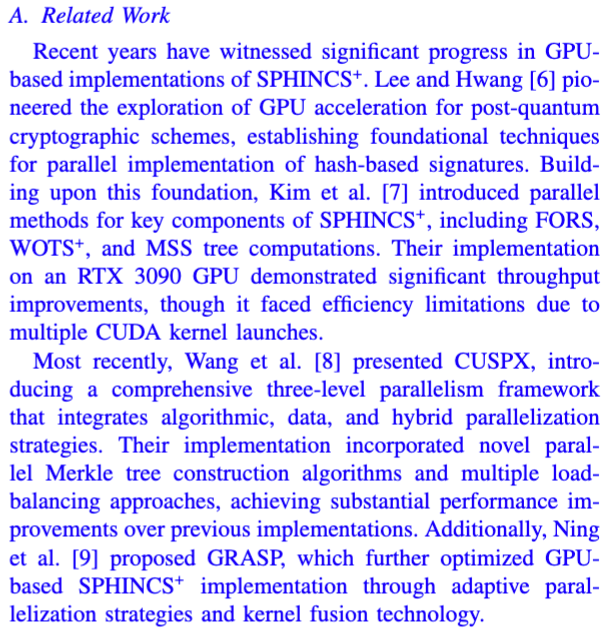
\includegraphics[width=\textwidth]{./fig/relate_work.png}
      \caption{相关工作部分}
      \label{fig:related_work}
    \end{subfigure}\hfill
    \begin{subfigure}[b]{0.32\textwidth}
      \centering
      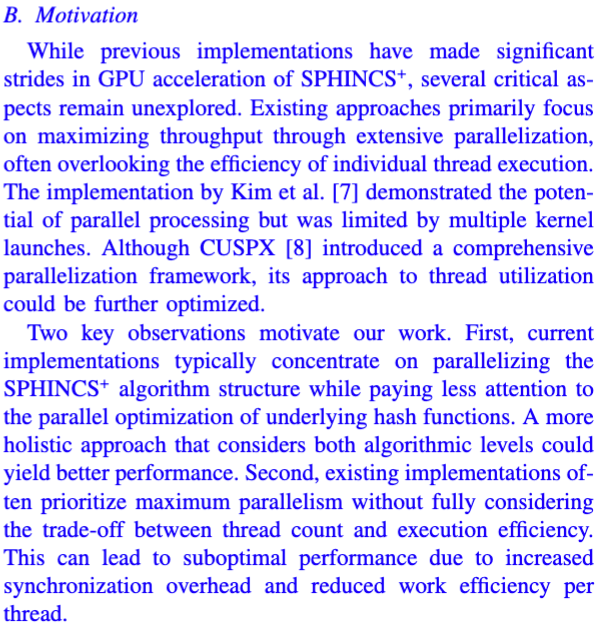
\includegraphics[width=\textwidth]{./fig/motivation.png}
      \caption{动机说明}
      \label{fig:motivation}
    \end{subfigure} \hfill
    \begin{subfigure}[b]{0.32\textwidth}
      \centering
      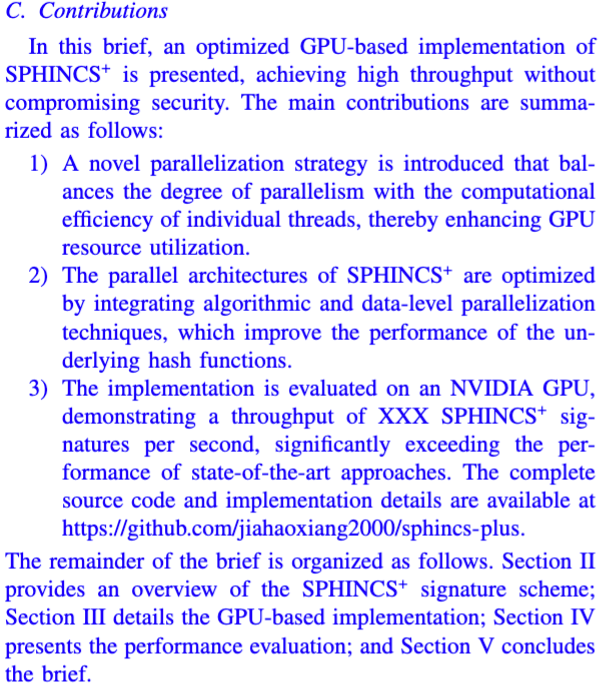
\includegraphics[width=\textwidth]{./fig/contributions.png}
      \caption{创新点部分}
      \label{fig:contributions}
    \end{subfigure}

    \caption{组合展示:相关工作、动机与创新点}
    \label{fig:composite}
  \end{figure}
\end{frame}

\begin{frame}
  \frametitle{老师评语}

  \begin{alertblock}{继续推进}

  \end{alertblock}

  \begin{block}{下周计划}
    1) GPU并行HASH函数设计与实现,降低延迟;

    2) 动态并行数调整策略,提高吞吐。
  \end{block}

\end{frame}

\begin{frame}
  \frametitle{参考文献}
  \bibliographystyle{alpha}
  \bibliography{../../paper}
\end{frame}

\end{document}
